% Options for packages loaded elsewhere
\PassOptionsToPackage{unicode}{hyperref}
\PassOptionsToPackage{hyphens}{url}
%
\documentclass[
  ,man,floatsintext]{apa6}
\usepackage{amsmath,amssymb}
\usepackage{iftex}
\ifPDFTeX
  \usepackage[T1]{fontenc}
  \usepackage[utf8]{inputenc}
  \usepackage{textcomp} % provide euro and other symbols
\else % if luatex or xetex
  \usepackage{unicode-math} % this also loads fontspec
  \defaultfontfeatures{Scale=MatchLowercase}
  \defaultfontfeatures[\rmfamily]{Ligatures=TeX,Scale=1}
\fi
\usepackage{lmodern}
\ifPDFTeX\else
  % xetex/luatex font selection
\fi
% Use upquote if available, for straight quotes in verbatim environments
\IfFileExists{upquote.sty}{\usepackage{upquote}}{}
\IfFileExists{microtype.sty}{% use microtype if available
  \usepackage[]{microtype}
  \UseMicrotypeSet[protrusion]{basicmath} % disable protrusion for tt fonts
}{}
\makeatletter
\@ifundefined{KOMAClassName}{% if non-KOMA class
  \IfFileExists{parskip.sty}{%
    \usepackage{parskip}
  }{% else
    \setlength{\parindent}{0pt}
    \setlength{\parskip}{6pt plus 2pt minus 1pt}}
}{% if KOMA class
  \KOMAoptions{parskip=half}}
\makeatother
\usepackage{xcolor}
\usepackage{graphicx}
\makeatletter
\def\maxwidth{\ifdim\Gin@nat@width>\linewidth\linewidth\else\Gin@nat@width\fi}
\def\maxheight{\ifdim\Gin@nat@height>\textheight\textheight\else\Gin@nat@height\fi}
\makeatother
% Scale images if necessary, so that they will not overflow the page
% margins by default, and it is still possible to overwrite the defaults
% using explicit options in \includegraphics[width, height, ...]{}
\setkeys{Gin}{width=\maxwidth,height=\maxheight,keepaspectratio}
% Set default figure placement to htbp
\makeatletter
\def\fps@figure{htbp}
\makeatother
\setlength{\emergencystretch}{3em} % prevent overfull lines
\providecommand{\tightlist}{%
  \setlength{\itemsep}{0pt}\setlength{\parskip}{0pt}}
\setcounter{secnumdepth}{-\maxdimen} % remove section numbering
% Make \paragraph and \subparagraph free-standing
\makeatletter
\ifx\paragraph\undefined\else
  \let\oldparagraph\paragraph
  \renewcommand{\paragraph}{
    \@ifstar
      \xxxParagraphStar
      \xxxParagraphNoStar
  }
  \newcommand{\xxxParagraphStar}[1]{\oldparagraph*{#1}\mbox{}}
  \newcommand{\xxxParagraphNoStar}[1]{\oldparagraph{#1}\mbox{}}
\fi
\ifx\subparagraph\undefined\else
  \let\oldsubparagraph\subparagraph
  \renewcommand{\subparagraph}{
    \@ifstar
      \xxxSubParagraphStar
      \xxxSubParagraphNoStar
  }
  \newcommand{\xxxSubParagraphStar}[1]{\oldsubparagraph*{#1}\mbox{}}
  \newcommand{\xxxSubParagraphNoStar}[1]{\oldsubparagraph{#1}\mbox{}}
\fi
\makeatother
% definitions for citeproc citations
\NewDocumentCommand\citeproctext{}{}
\NewDocumentCommand\citeproc{mm}{%
  \begingroup\def\citeproctext{#2}\cite{#1}\endgroup}
\makeatletter
 % allow citations to break across lines
 \let\@cite@ofmt\@firstofone
 % avoid brackets around text for \cite:
 \def\@biblabel#1{}
 \def\@cite#1#2{{#1\if@tempswa , #2\fi}}
\makeatother
\newlength{\cslhangindent}
\setlength{\cslhangindent}{1.5em}
\newlength{\csllabelwidth}
\setlength{\csllabelwidth}{3em}
\newenvironment{CSLReferences}[2] % #1 hanging-indent, #2 entry-spacing
 {\begin{list}{}{%
  \setlength{\itemindent}{0pt}
  \setlength{\leftmargin}{0pt}
  \setlength{\parsep}{0pt}
  % turn on hanging indent if param 1 is 1
  \ifodd #1
   \setlength{\leftmargin}{\cslhangindent}
   \setlength{\itemindent}{-1\cslhangindent}
  \fi
  % set entry spacing
  \setlength{\itemsep}{#2\baselineskip}}}
 {\end{list}}
\usepackage{calc}
\newcommand{\CSLBlock}[1]{\hfill\break\parbox[t]{\linewidth}{\strut\ignorespaces#1\strut}}
\newcommand{\CSLLeftMargin}[1]{\parbox[t]{\csllabelwidth}{\strut#1\strut}}
\newcommand{\CSLRightInline}[1]{\parbox[t]{\linewidth - \csllabelwidth}{\strut#1\strut}}
\newcommand{\CSLIndent}[1]{\hspace{\cslhangindent}#1}
\ifLuaTeX
\usepackage[bidi=basic]{babel}
\else
\usepackage[bidi=default]{babel}
\fi
\babelprovide[main,import]{english}
% get rid of language-specific shorthands (see #6817):
\let\LanguageShortHands\languageshorthands
\def\languageshorthands#1{}
% Manuscript styling
\usepackage{upgreek}
\captionsetup{font=singlespacing,justification=justified}

% Table formatting
\usepackage{longtable}
\usepackage{lscape}
% \usepackage[counterclockwise]{rotating}   % Landscape page setup for large tables
\usepackage{multirow}		% Table styling
\usepackage{tabularx}		% Control Column width
\usepackage[flushleft]{threeparttable}	% Allows for three part tables with a specified notes section
\usepackage{threeparttablex}            % Lets threeparttable work with longtable

% Create new environments so endfloat can handle them
% \newenvironment{ltable}
%   {\begin{landscape}\centering\begin{threeparttable}}
%   {\end{threeparttable}\end{landscape}}
\newenvironment{lltable}{\begin{landscape}\centering\begin{ThreePartTable}}{\end{ThreePartTable}\end{landscape}}

% Enables adjusting longtable caption width to table width
% Solution found at http://golatex.de/longtable-mit-caption-so-breit-wie-die-tabelle-t15767.html
\makeatletter
\newcommand\LastLTentrywidth{1em}
\newlength\longtablewidth
\setlength{\longtablewidth}{1in}
\newcommand{\getlongtablewidth}{\begingroup \ifcsname LT@\roman{LT@tables}\endcsname \global\longtablewidth=0pt \renewcommand{\LT@entry}[2]{\global\advance\longtablewidth by ##2\relax\gdef\LastLTentrywidth{##2}}\@nameuse{LT@\roman{LT@tables}} \fi \endgroup}

% \setlength{\parindent}{0.5in}
% \setlength{\parskip}{0pt plus 0pt minus 0pt}

% Overwrite redefinition of paragraph and subparagraph by the default LaTeX template
% See https://github.com/crsh/papaja/issues/292
\makeatletter
\renewcommand{\paragraph}{\@startsection{paragraph}{4}{\parindent}%
  {0\baselineskip \@plus 0.2ex \@minus 0.2ex}%
  {-1em}%
  {\normalfont\normalsize\bfseries\itshape\typesectitle}}

\renewcommand{\subparagraph}[1]{\@startsection{subparagraph}{5}{1em}%
  {0\baselineskip \@plus 0.2ex \@minus 0.2ex}%
  {-\z@\relax}%
  {\normalfont\normalsize\itshape\hspace{\parindent}{#1}\textit{\addperi}}{\relax}}
\makeatother

\makeatletter
\usepackage{etoolbox}
\patchcmd{\maketitle}
  {\section{\normalfont\normalsize\abstractname}}
  {\section*{\normalfont\normalsize\abstractname}}
  {}{\typeout{Failed to patch abstract.}}
\patchcmd{\maketitle}
  {\section{\protect\normalfont{\@title}}}
  {\section*{\protect\normalfont{\@title}}}
  {}{\typeout{Failed to patch title.}}
\makeatother

\usepackage{xpatch}
\makeatletter
\xapptocmd\appendix
  {\xapptocmd\section
    {\addcontentsline{toc}{section}{\appendixname\ifoneappendix\else~\theappendix\fi: #1}}
    {}{\InnerPatchFailed}%
  }
{}{\PatchFailed}
\makeatother
\keywords{keywords\newline\indent Word count: X}
\usepackage{csquotes}
\usepackage[titles]{tocloft}
\cftpagenumbersoff{figure}
\renewcommand{\cftfigpresnum}{\itshape\figurename\enspace}
\renewcommand{\cftfigaftersnum}{.\space}
\setlength{\cftfigindent}{0pt}
\setlength{\cftafterloftitleskip}{0pt}
\settowidth{\cftfignumwidth}{Figure 10.\qquad}
\cftpagenumbersoff{table}
\renewcommand{\cfttabpresnum}{\itshape\tablename\enspace}
\renewcommand{\cfttabaftersnum}{.\space}
\setlength{\cfttabindent}{0pt}
\setlength{\cftafterloftitleskip}{0pt}
\settowidth{\cfttabnumwidth}{Table 10.\qquad}
\ifLuaTeX
  \usepackage{selnolig}  % disable illegal ligatures
\fi
\usepackage{bookmark}
\IfFileExists{xurl.sty}{\usepackage{xurl}}{} % add URL line breaks if available
\urlstyle{same}
\hypersetup{
  pdftitle={Variation of {[}v{]} in Cook Islands Māori},
  pdfauthor={Quartz ColvinRutgers University},
  pdflang={en-EN},
  pdfkeywords={keywords},
  hidelinks,
  pdfcreator={LaTeX via pandoc}}

\title{Variation of {[}v{]} in Cook Islands Māori}
\author{Quartz Colvin\textsuperscript{Rutgers University}}
\date{}


\shorttitle{Cook Islands Māori}

\affiliation{\phantom{0}}

\begin{document}
\maketitle

\section{1.0 Introduction}\label{introduction}

In this paper, we will do a statistical analysis of {[}v{]} across a sample of islands in Cook Islands Māori (CIM). It's known that in many dialects and other varieties of Māori, this phoneme can be realized as {[}w{]} or {[}v{]}. This paper aims to take a statistical approach to this generalization.

This paper has four sub-questions to investigate. First, how does w\textasciitilde v duration vary by island and second, how does intensity for these phonemes vary by island. The other two questions are about identifying information about the surface forms of w\textasciitilde v by island. Specifically, we will model f0 and f2 to determine whether certain islands have a voiced phoneme realized. Finally, the f2 model will help us determine which islands have higher rates of {[}w{]}s surfacing and which have more {[}v{]}s surfacing.

\subsection{1.1 Background (CIM)}\label{background-cim}

Cook Islands Māori is an Eastern Polynesian language classified as \emph{Endangered}. It is very closely related to Aotearoa Māori, but is definitely different from it.

It's known across both Aotearoa (NZ) Māori and CIM that some speakers regularly pronounce {[}v{]} as {[}w{]}, but it isn't clear to anyone who does this more and what conditions it.

\textbf{???fill in}

\section{2.0 Methods}\label{methods}

\textbf{???fill in}

\section{3.0 Data}\label{data}

\textbf{???fill in}

\section{4.0 Analysis}\label{analysis}

This section readdresses the main questions about the w\textasciitilde v alternation. First, how does duration differ by island and second, how does intensity vary by island? Finally, do any islands have regular occurrence of {[}w{]} instead of {[}v{]} surfacing. For this final question, we will compare f0 and f2 separately.

Note that in all of my models, I did not control for where w\textasciitilde v occurs in the word, since I am looking at general frequency information and not doing a phonological analysis of specific environments in which {[}w{]} or {[}v{]} occurs more.

???discuss autocorrelation issue

\subsection{4.1 Duration by island}\label{duration-by-island}

\textbf{???fill in}

\begin{tabular}{l|l|l|r}
\hline
speaker & island & word & duration\\
\hline
TA & Atiu & ava & 0.08\\
\hline
TA & Atiu & ava & 0.07\\
\hline
TA & Atiu & ava & 0.14\\
\hline
TA & Atiu & ava & 0.11\\
\hline
TA & Atiu & ava & 0.05\\
\hline
TA & Atiu & ava & 0.13\\
\hline
\end{tabular}

\begin{figure}
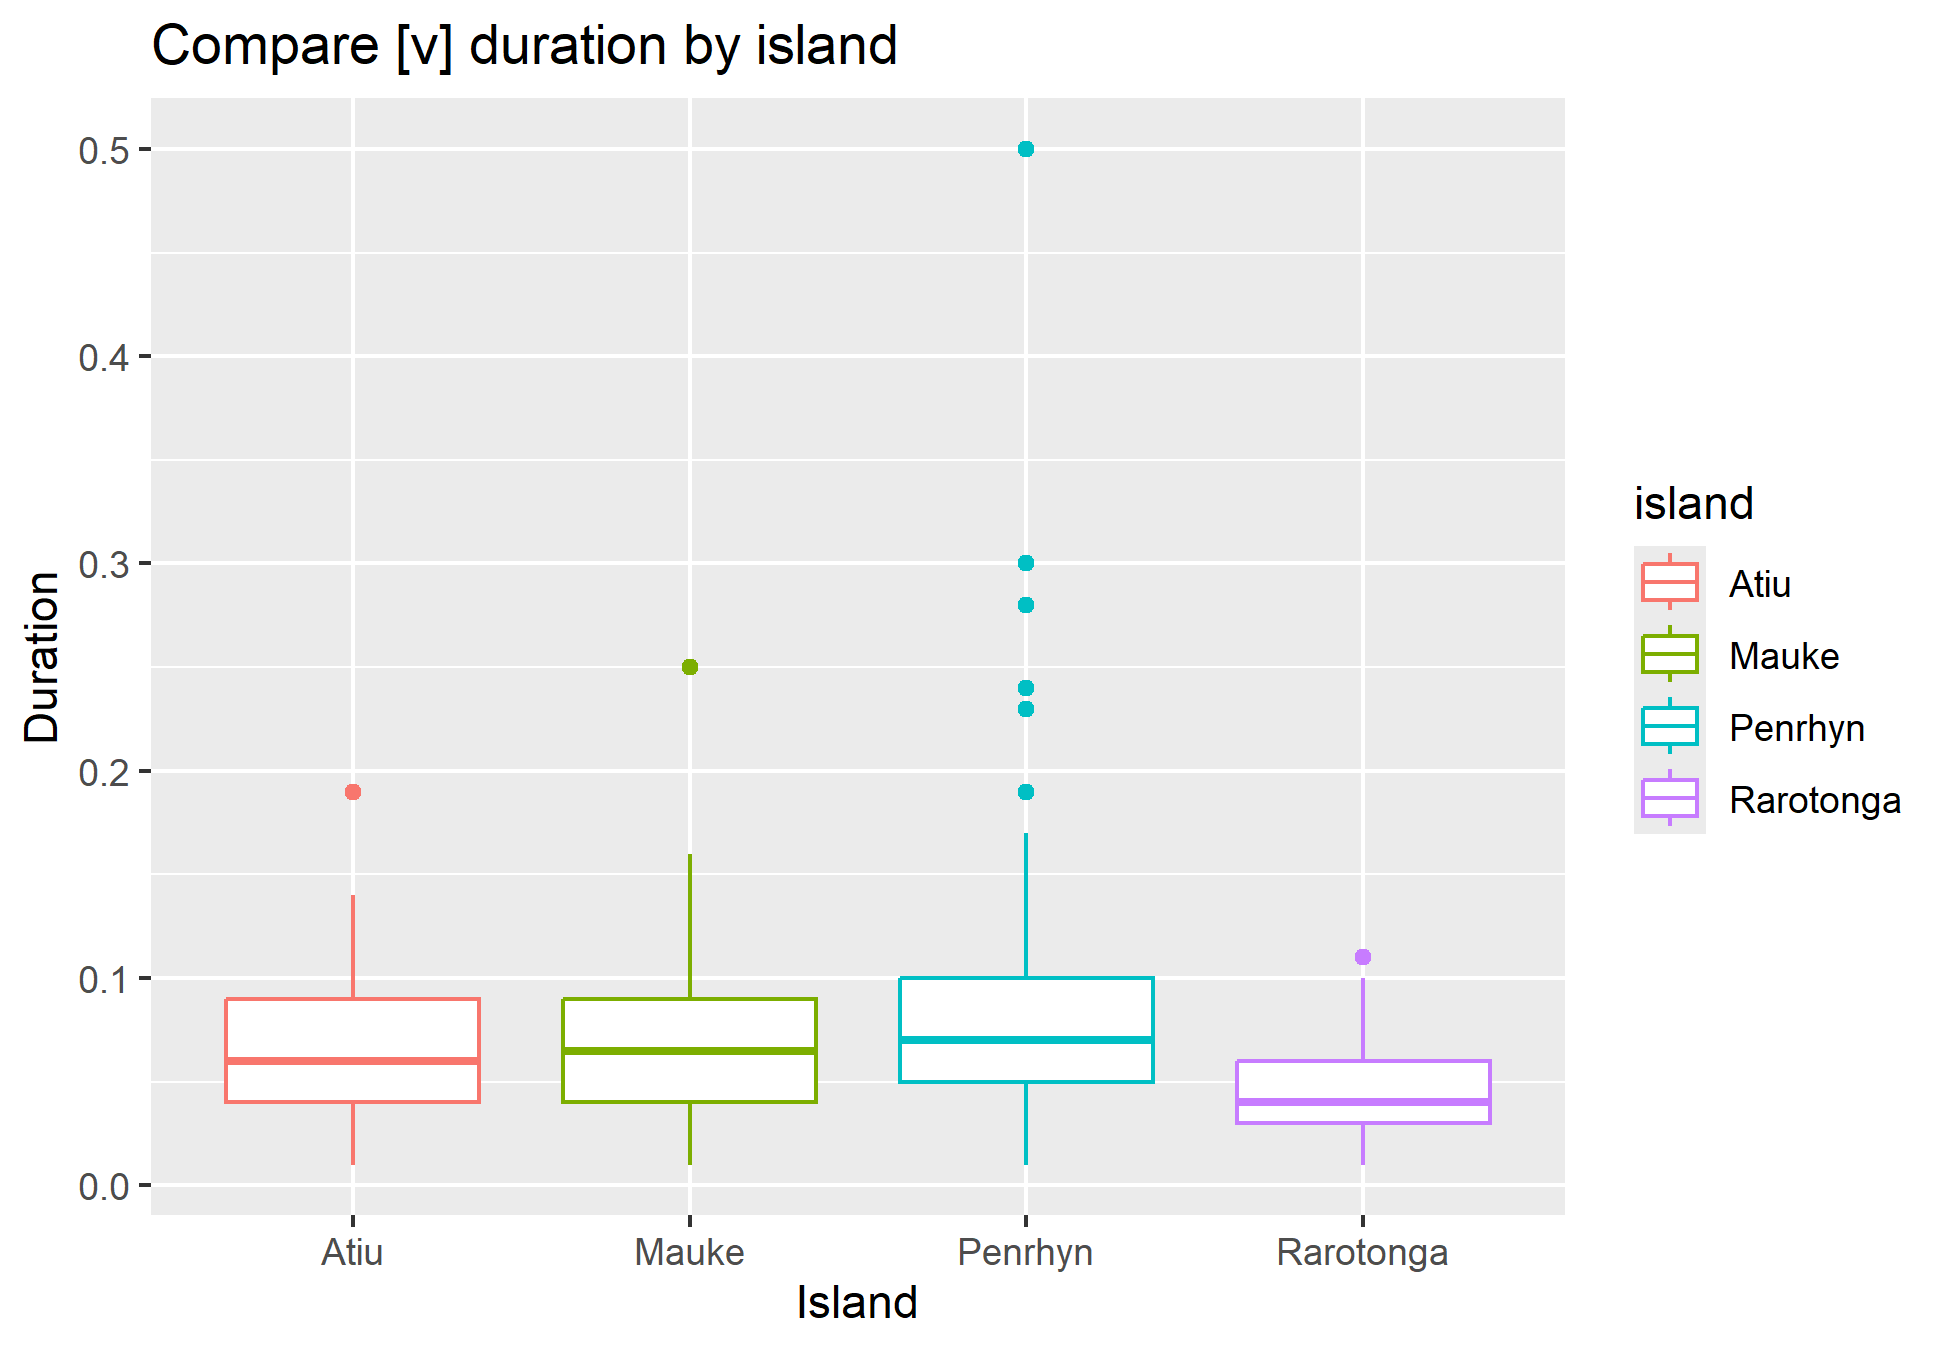
\includegraphics[width=0.75\linewidth]{D2_CIM_files/figure-latex/print-duration-plot-1} \caption{ }\label{fig:print-duration-plot}
\end{figure}

\begin{tabular}{l|r|r|r|r}
\hline
term & estimate & std.error & statistic & p.value\\
\hline
(Intercept) & 0.0660169 & 0.0033898 & 19.4750727 & 0.0000000\\
\hline
islandMauke & -0.0003532 & 0.0038067 & -0.0927931 & 0.9260887\\
\hline
islandPenrhyn & 0.0179242 & 0.0044121 & 4.0624899 & 0.0000528\\
\hline
islandRarotonga & -0.0208246 & 0.0044925 & -4.6354104 & 0.0000041\\
\hline
\end{tabular}

\subsection{4.2 Intensity by island}\label{intensity-by-island}

\textbf{???fill in}

\begin{tabular}{l|l|l|r}
\hline
speaker & island & word & intensity\\
\hline
TA & Atiu & ava & 54.08202\\
\hline
TA & Atiu & ava & 58.06061\\
\hline
TA & Atiu & ava & 48.40481\\
\hline
TA & Atiu & ava & 54.18315\\
\hline
TA & Atiu & ava & 49.59224\\
\hline
TA & Atiu & ava & 53.07335\\
\hline
\end{tabular}

\begin{figure}
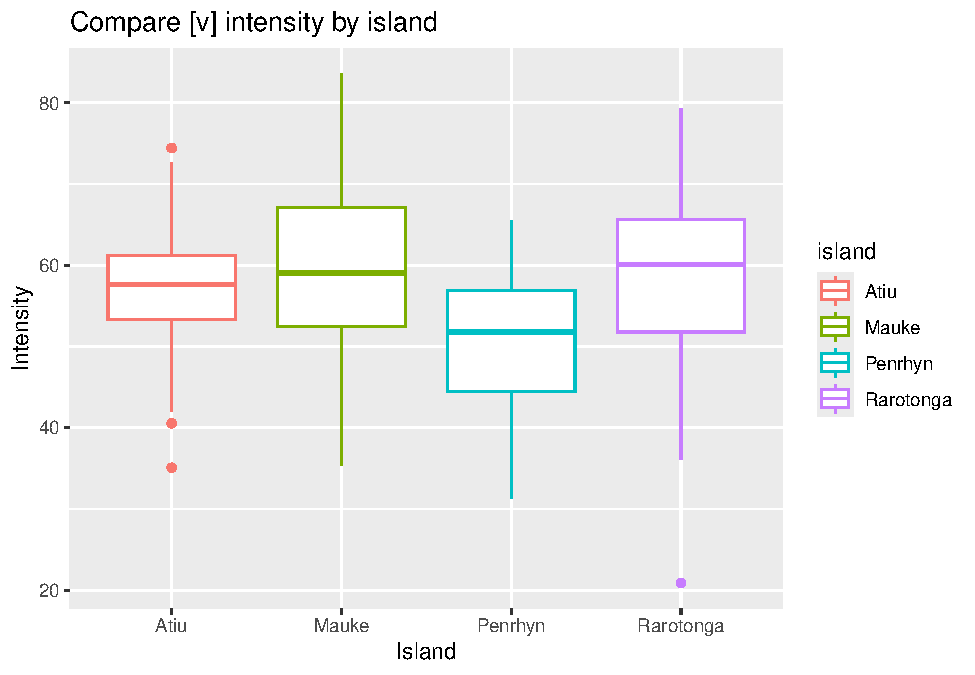
\includegraphics[width=0.75\linewidth]{D2_CIM_files/figure-latex/print-intensity-plot-1} \caption{ }\label{fig:print-intensity-plot}
\end{figure}

\begin{tabular}{l|r|r|r|r}
\hline
term & estimate & std.error & statistic & p.value\\
\hline
(Intercept) & 57.4682172 & 0.8418656 & 68.2629370 & 0.0000000\\
\hline
islandMauke & 2.2841738 & 0.9458247 & 2.4150075 & 0.0159356\\
\hline
islandPenrhyn & -6.9840858 & 1.0957577 & -6.3737500 & 0.0000000\\
\hline
islandRarotonga & 0.0787305 & 1.1157213 & 0.0705647 & 0.9437601\\
\hline
\end{tabular}

\subsection{4.3 Voicing by island}\label{voicing-by-island}

\textbf{???fill in}

\begin{tabular}{l|l|l|r|r}
\hline
speaker & island & word & f0 & duration\\
\hline
TA & Atiu & ava & 128.5916 & 0.08\\
\hline
TA & Atiu & ava & 127.0908 & 0.08\\
\hline
TA & Atiu & ava & 127.4540 & 0.08\\
\hline
TA & Atiu & ava & 160.6464 & 0.07\\
\hline
TA & Atiu & ava & 157.4397 & 0.07\\
\hline
TA & Atiu & ava & 158.2820 & 0.07\\
\hline
\end{tabular}

\begin{figure}
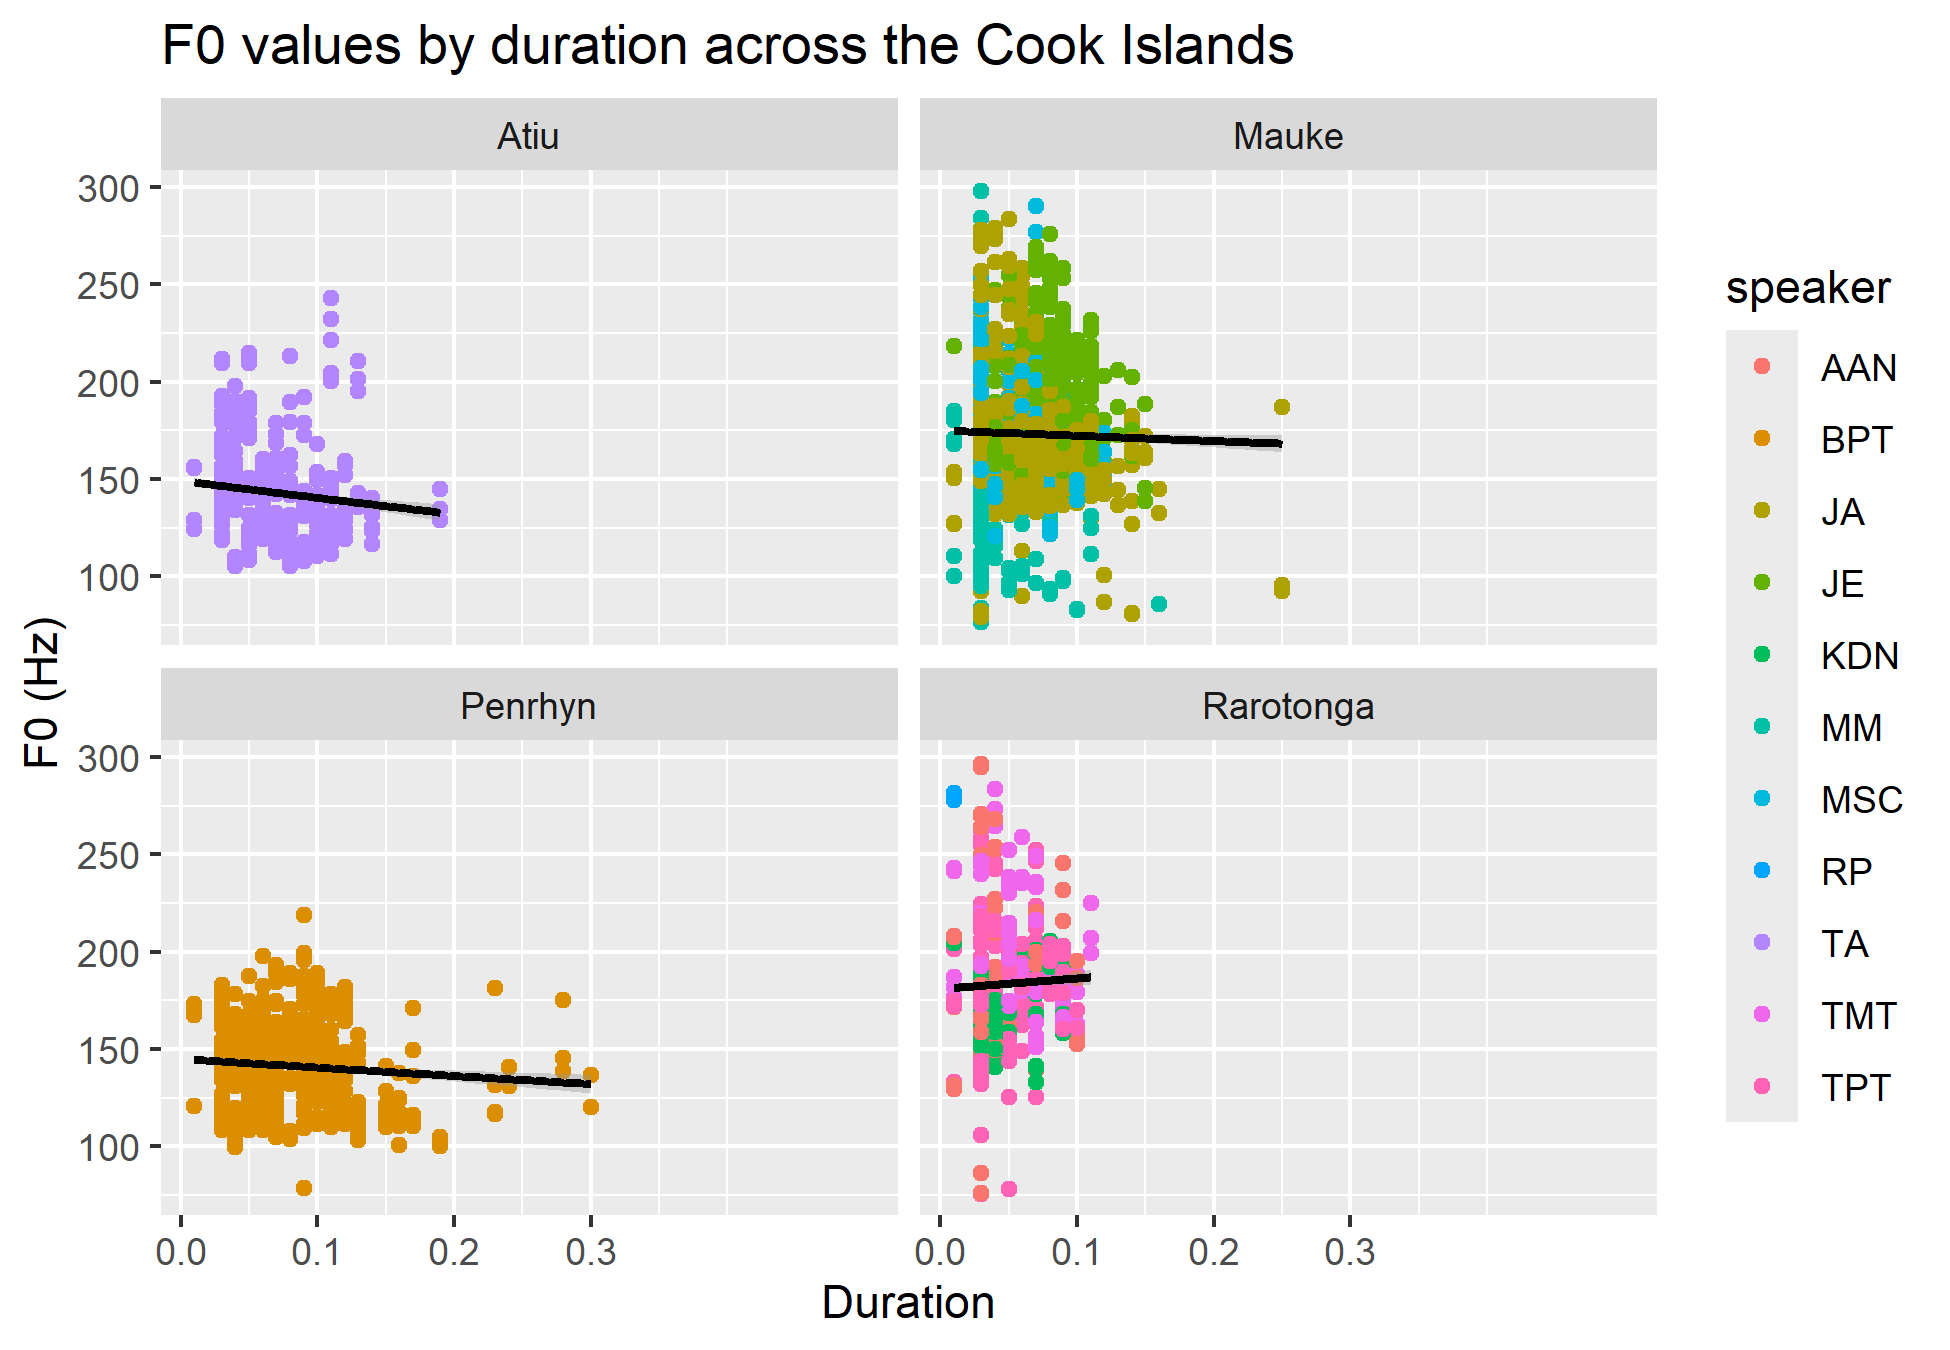
\includegraphics[width=0.75\linewidth]{D2_CIM_files/figure-latex/plot-f0-1} \caption{ }\label{fig:plot-f0}
\end{figure}

\begin{tabular}{l|r|r|r|r}
\hline
term & estimate & std.error & statistic & p.value\\
\hline
(Intercept) & 143.226548 & 1.779445 & 80.4894349 & 0.0000000\\
\hline
islandMauke & 29.922893 & 2.005496 & 14.9204478 & 0.0000000\\
\hline
islandPenrhyn & -1.840639 & 2.304081 & -0.7988602 & 0.4244468\\
\hline
islandRarotonga & 40.179828 & 2.400413 & 16.7387166 & 0.0000000\\
\hline
\end{tabular}

\subsection{4.4 w\textasciitilde v distribution by island}\label{wv-distribution-by-island}

\textbf{???fill in}

\begin{tabular}{l|l|l|r}
\hline
speaker & island & word & f2\\
\hline
TA & Atiu & ava & 964.3925\\
\hline
TA & Atiu & ava & 950.2333\\
\hline
TA & Atiu & ava & 2575.9621\\
\hline
TA & Atiu & ava & 961.5736\\
\hline
TA & Atiu & ava & 984.4541\\
\hline
TA & Atiu & ava & 896.0441\\
\hline
\end{tabular}

\begin{figure}
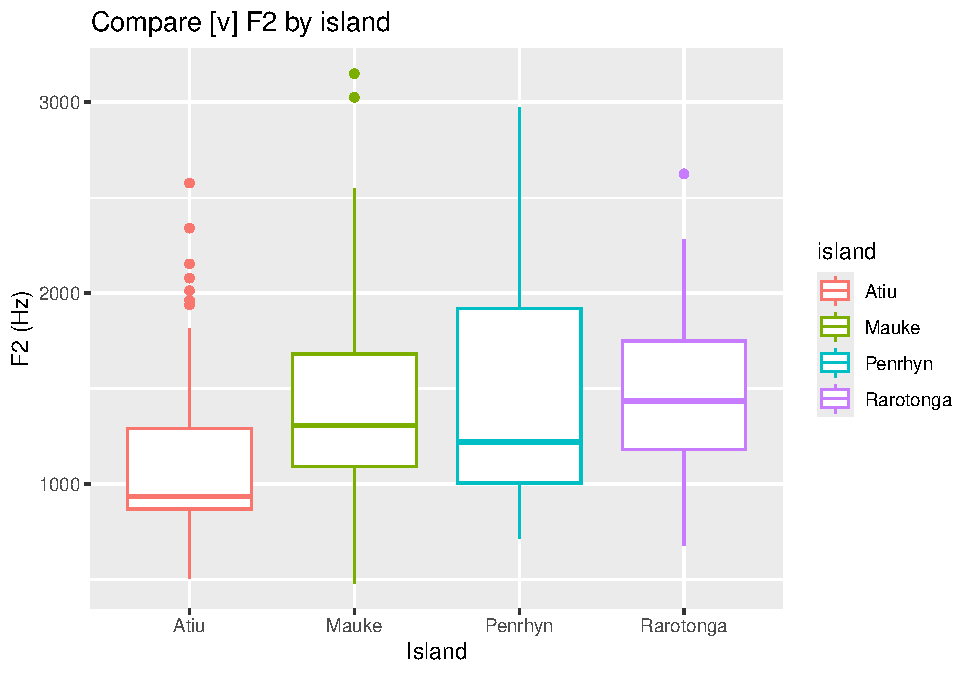
\includegraphics[width=0.75\linewidth]{D2_CIM_files/figure-latex/plot-f2-1} \caption{ }\label{fig:plot-f2}
\end{figure}

\begin{tabular}{l|r|r|r|r}
\hline
term & estimate & std.error & statistic & p.value\\
\hline
(Intercept) & 1090.9432 & 39.79288 & 27.415534 & 0\\
\hline
islandMauke & 308.5190 & 44.70677 & 6.900944 & 0\\
\hline
islandPenrhyn & 373.9431 & 51.79373 & 7.219853 & 0\\
\hline
islandRarotonga & 360.9223 & 52.73736 & 6.843768 & 0\\
\hline
\end{tabular}

\subsection{5.1 Data analysis}\label{data-analysis}

I used R (Version 4.5.0; R Core Team, 2024) and the R-packages \emph{broom} (Version 1.0.8; Robinson, Hayes, \& Couch, 2025), \emph{dplyr} (Version 1.1.4; Wickham, François, Henry, Müller, \& Vaughan, 2023), \emph{ds4ling} (Version 1.0; Casillas, 2025), \emph{forcats} (Version 1.0.0; Wickham, 2023a), \emph{ggplot2} (Version 3.5.2; Wickham, 2016), \emph{ggpubr} (Version 0.6.0; Kassambara, 2023), \emph{here} (Version 1.0.1; Müller, 2020), \emph{lme4} (Version 1.1.37; Bates, Mächler, Bolker, \& Walker, 2015), \emph{lmerTest} (Version 3.1.3; Kuznetsova, Brockhoff, \& Christensen, 2017), \emph{lubridate} (Version 1.9.4; Grolemund \& Wickham, 2011), \emph{Matrix} (Version 1.7.3; Bates, Maechler, \& Jagan, 2025), \emph{papaja} (Version 0.1.3; Aust \& Barth, 2024), \emph{purrr} (Version 1.0.4; Wickham \& Henry, 2025), \emph{readr} (Version 2.1.5; Wickham, Hester, \& Bryan, 2024), \emph{stringr} (Version 1.5.1; Wickham, 2023b), \emph{tibble} (Version 3.2.1; Müller \& Wickham, 2023), \emph{tidyr} (Version 1.3.1; Wickham, Vaughan, \& Girlich, 2024), \emph{tidyverse} (Version 2.0.0; Wickham et al., 2019) and \emph{tinylabels} (Version 0.2.5; Barth, 2023) for all my analyses.

\section{6.0 Conclusion}\label{conclusion}

???fill in

\section{References}\label{references}

\setlength{\parindent}{-0.5in}
\setlength{\leftskip}{0.5in}

\phantomsection\label{refs}
\begin{CSLReferences}{1}{0}
\bibitem[\citeproctext]{ref-R-papaja}
Aust, F., \& Barth, M. (2024). \emph{{papaja}: {Prepare} reproducible {APA} journal articles with {R Markdown}}. \url{https://doi.org/10.32614/CRAN.package.papaja}

\bibitem[\citeproctext]{ref-R-tinylabels}
Barth, M. (2023). \emph{{tinylabels}: Lightweight variable labels}. Retrieved from \url{https://cran.r-project.org/package=tinylabels}

\bibitem[\citeproctext]{ref-R-lme4}
Bates, D., Mächler, M., Bolker, B., \& Walker, S. (2015). Fitting linear mixed-effects models using {lme4}. \emph{Journal of Statistical Software}, \emph{67}(1), 1--48. \url{https://doi.org/10.18637/jss.v067.i01}

\bibitem[\citeproctext]{ref-R-Matrix}
Bates, D., Maechler, M., \& Jagan, M. (2025). \emph{Matrix: Sparse and dense matrix classes and methods}. \url{https://doi.org/10.32614/CRAN.package.Matrix}

\bibitem[\citeproctext]{ref-R-ds4ling}
Casillas, J. (2025). \emph{ds4ling: Datasets and functions developed for SPAN658: Data science for linguists}. Retrieved from \url{https://github.com/jvcasillas/ds4ling}

\bibitem[\citeproctext]{ref-R-lubridate}
Grolemund, G., \& Wickham, H. (2011). Dates and times made easy with {lubridate}. \emph{Journal of Statistical Software}, \emph{40}(3), 1--25. Retrieved from \url{https://www.jstatsoft.org/v40/i03/}

\bibitem[\citeproctext]{ref-R-ggpubr}
Kassambara, A. (2023). \emph{Ggpubr: 'ggplot2' based publication ready plots}. \url{https://doi.org/10.32614/CRAN.package.ggpubr}

\bibitem[\citeproctext]{ref-R-lmerTest}
Kuznetsova, A., Brockhoff, P. B., \& Christensen, R. H. B. (2017). {lmerTest} package: Tests in linear mixed effects models. \emph{Journal of Statistical Software}, \emph{82}(13), 1--26. \url{https://doi.org/10.18637/jss.v082.i13}

\bibitem[\citeproctext]{ref-R-here}
Müller, K. (2020). \emph{Here: A simpler way to find your files}. \url{https://doi.org/10.32614/CRAN.package.here}

\bibitem[\citeproctext]{ref-R-tibble}
Müller, K., \& Wickham, H. (2023). \emph{Tibble: Simple data frames}. \url{https://doi.org/10.32614/CRAN.package.tibble}

\bibitem[\citeproctext]{ref-R-base}
R Core Team. (2024). \emph{R: A language and environment for statistical computing}. Vienna, Austria: R Foundation for Statistical Computing. Retrieved from \url{https://www.R-project.org/}

\bibitem[\citeproctext]{ref-R-broom}
Robinson, D., Hayes, A., \& Couch, S. (2025). \emph{Broom: Convert statistical objects into tidy tibbles}. \url{https://doi.org/10.32614/CRAN.package.broom}

\bibitem[\citeproctext]{ref-R-ggplot2}
Wickham, H. (2016). \emph{ggplot2: Elegant graphics for data analysis}. Springer-Verlag New York. Retrieved from \url{https://ggplot2.tidyverse.org}

\bibitem[\citeproctext]{ref-R-forcats}
Wickham, H. (2023a). \emph{Forcats: Tools for working with categorical variables (factors)}. \url{https://doi.org/10.32614/CRAN.package.forcats}

\bibitem[\citeproctext]{ref-R-stringr}
Wickham, H. (2023b). \emph{Stringr: Simple, consistent wrappers for common string operations}. \url{https://doi.org/10.32614/CRAN.package.stringr}

\bibitem[\citeproctext]{ref-R-tidyverse}
Wickham, H., Averick, M., Bryan, J., Chang, W., McGowan, L. D., François, R., \ldots{} Yutani, H. (2019). Welcome to the {tidyverse}. \emph{Journal of Open Source Software}, \emph{4}(43), 1686. \url{https://doi.org/10.21105/joss.01686}

\bibitem[\citeproctext]{ref-R-dplyr}
Wickham, H., François, R., Henry, L., Müller, K., \& Vaughan, D. (2023). \emph{Dplyr: A grammar of data manipulation}. \url{https://doi.org/10.32614/CRAN.package.dplyr}

\bibitem[\citeproctext]{ref-R-purrr}
Wickham, H., \& Henry, L. (2025). \emph{Purrr: Functional programming tools}. \url{https://doi.org/10.32614/CRAN.package.purrr}

\bibitem[\citeproctext]{ref-R-readr}
Wickham, H., Hester, J., \& Bryan, J. (2024). \emph{Readr: Read rectangular text data}. \url{https://doi.org/10.32614/CRAN.package.readr}

\bibitem[\citeproctext]{ref-R-tidyr}
Wickham, H., Vaughan, D., \& Girlich, M. (2024). \emph{Tidyr: Tidy messy data}. \url{https://doi.org/10.32614/CRAN.package.tidyr}

\end{CSLReferences}


\clearpage
\renewcommand{\listfigurename}{Figure captions}

\clearpage
\renewcommand{\listtablename}{Table captions}


\end{document}
